%%This is a very basic article template.
%%There is just one section and two subsections.
\documentclass[11pt]{article}
\usepackage[T1]{fontenc}
\usepackage[utf8]{inputenc}
\usepackage[ngerman]{babel}
\usepackage{natbib}
\usepackage[onehalfspacing]{setspace}
\usepackage{geometry}
\usepackage[scaled]{uarial}
\usepackage{graphicx}
\usepackage{float}
\usepackage{amssymb}
\usepackage{amsmath}


\usepackage{inconsolata}

\usepackage{color}

\definecolor{pblue}{rgb}{0.13,0.13,1}
\definecolor{pgreen}{rgb}{0,0.5,0}
\definecolor{pred}{rgb}{0.9,0,0}
\definecolor{pgrey}{rgb}{0.46,0.45,0.48}

\usepackage{listings}
\lstset{language=Java,
  showspaces=false,
  showtabs=false,
  breaklines=true,
  showstringspaces=false,
  breakatwhitespace=true,
  commentstyle=\color{pgreen},
  keywordstyle=\color{pblue},
  stringstyle=\color{pred},
  basicstyle=\ttfamily,
  moredelim=[il][\textcolor{pgrey}]{$$},
  moredelim=[is][\textcolor{pgrey}]{\%\%}{\%\%}
}


\bibliographystyle{plainnat}
\geometry{a4paper, top=25mm, left=40mm, right=20mm, bottom=25mm}
\begin{document}
\begin{onehalfspacing}
\subsection{Abgrenzung zu nicht-relationalen Datenbanken}
Der Markt der Datenbanksysteme ist riesig und es existieren mehrere verschiedene
Konzeptionsmethoden von Datenbanken. Neben den relationalen Datenbanken sind
nicht-relationale Datenbanken eine weitverbreitete Technik zur Speicherung von
Datenmengen. \\

Nicht-relationale Datenbanken (oder auch NOSQL-Datenbanken - "`Not Only SQL"')
verfolgen eine andere Zielsetzung als relationale Datenbanken. Folgende
Abbildung illustriert die unterschiedlichen Ziele.
\begin{figure}[H]
\centering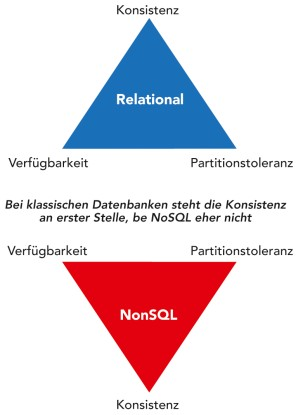
\includegraphics[width=0.6\textwidth]{NoSQL.jpg}
\caption[Zielunterschiede Relationale vs. Nicht-Relationale
Datenbanken]{grafische Darstellung der Zielunterschiede zwischen Relationale und
Nicht-Relationale Datenbanken - Quelle:
http://www.computerwoche.de/a/nosql-die-neue-alte-datenbank-generation,2497315,3,
Stand 17.03.2016}
\end{figure}
Wie man der Abbildung entnehmen kann, sind bei NoSQL-Datenbanken Verfügbarkeit
und Partitionstoleranz wichtiger als Konsistenz, welches bei relationalen
Datenbanken das wichtigste Ziel darstellt. Geschuldet ist diese Zielpolitik der
führen Entwicklung der ersten Applikationen für das Internet. Damals war die
Hardware der technischen Geräte bei weitem nicht in der Leistungsklasse wie
heutzutage. Viele Smartphones aus dem Jahre 2015 verfügen über weit mehr
Rechenleistung wie Server aus der damaligen Zeit. \\
Als früher die Datenbanksätze sehr groß wurden, schlug dies auf die Performance
der Anwendungen nieder. Lange Zugriffzeiten waren vorprogrammiert, welche vor
allem in Web-Applikationen für viel Frust sorgten. Daraufhin setzten sich
Menschen zusammen und überlegten sich ein neues Modellierungskonzept: das
Resultat sind die nicht-relationalen Datenbanken. Sie zeichnen sich durch
folgende Kriterien aus:
\begin{itemize}
  \item Datenbankmodell nicht relational: in bestimmten Anwendungsfällen bessere
  Performance
  \item Verteilte und horizontale Skalierbarkeit: effektivere Skalierung und
  Verteilung
  \item (Fast) Schemafrei: Zugewinn an Flexibilität
  \item Einfache Programmierschnittstelle: Durch die geringe Befehlsvielfalt in
  SQL sind detailierte Abfragen sehr komplex. NoSQL-Datenbanken stellen immer
  eine Andockstelle für Programmiersprachen bereit, wie z.B. MongoDB für
  Javascript
  \item Konsistenzmodell nicht ACID (Atomicity, Consistency, Isolation,
  Durability): Der wohl wichtigste Unterscheidungspunkt. Während relationale
  Datenbanken um jeden Preis sicherstellen, dass Daten zu jedem Zeitpunkt
  konsistent und richtig sind, agieren NoSQL-Datenbanken nach dem BASE-Prinzip
  (Basically Avaiable, Soft State, Eventually Consistent). Mit dem Base-Prinzip
  liegt der Fokus auf die Verfügbarkeit von Daten und weniger auf die Konsistenz
  dieser.
\end{itemize}
Bekannte Datenbanksysteme, die auf NoSQL-Kriterien aufbauen sind:
\begin{itemize}
  \item Key/Value-Datenbanksysteme
  \item Spaltenorientierte Datenbanksysteme
  \item Dokumentenorientierte Datenbanksysteme
  \item Graphendatenbanken
\end{itemize}
Letzter Punkt wäre ebenfalls eine Möglichkeit, das Parkleitsystem dieses
Projektes zu verwalten, jedoch wurde sich auf Grund der Einfachheit der
Installtion für ein relationales Datenbanksystem entschieden.
\subsection{Implementierung einer SQLite3-Datenbank in Android}
Android, ein mobiles Betriebssystem welches auf der Programmiersprache Java
aufbaut, bietet eine einfache Speicherung und Verwaltung von persistenten Daten
durch eine SQLite3-Datenbank an. SQLite gehört zu den relationalen
Datenbanksystemen. \\

Dieses Projekt beinhaltet eine eigene Klasse namens "`DatabaseHandler"'. Diese
regelt die Operationen auf der Datenbank und bildet die zentrale Schnittstelle
für die Anwendung.\\
Am Anfang der Klasse werden zuerst generelle Paramter festgelegt, hierzu gehören
Namen der Datenbank und Version des Datenbankschemas.
\begin{lstlisting}
//DECLARE GENERAL-PARAMETERS
public static final String DB_NAME = "database.SQLite";
public static final int DB_VERSION = 1;
\end{lstlisting}
Danach wird die Struktur der einzelnen Tabellen definiert.
\begin{lstlisting}
//DECLARE COLUMNS-PARKING
public static final String TB_NAME_PARKING = "parking";
public static final String SPACE_PARKING = "SPACE";
public static final String _FREE = "_FREE";
public static final String _GROUP_PARK = "_GROUP";

//DECLARE COLUMNS-GROUPS
public static final String TB_NAME_GROUPS = "groups";
public static final String ID = "ID";
public static final String _GROUP_GROUPS = "_GROUP";

//DECLARE COLUMNS-PARKING
public static final String TB_NAME_PARKING_COLOR = "parking_color";
public static final String SPACE_PARKING_COLOR = "SPACE";
public static final String _COLOR_LEFT = "COLOR_LEFT";
public static final String _COLOR_RIGHT = "COLOR_RIGHT";
\end{lstlisting}

Spaltennamen welche einen Unterstrich vor sich führen besitzen keine besondere
Wertung, sondern korrelieren sonst mit reservierten Wörtern der Sprache SQL. \\

Die Tabellen wurden hierdurch jedoch noch nicht automatisch kreiert (auch nicht
bei Programmstart), sondern müssen vorerst noch mittels String im System erzeugt
werden. Hierbei können direkt weitere Integritätsbedingungen der Tabellen
festgelegt werden (Primärschlüssel, Fremdschlüssel, "`nicht null"',\ldots). 
\begin{lstlisting}
//CREATE PARKING-TABLE
String CREATE_PARKING_TABLE = "CREATE TABLE IF NOT EXISTS " + TB_NAME_PARKING
		+ " (" 
		+ SPACE_PARKING + " INTEGER PRIMARY KEY NOT NULL,"
		+ _FREE + " INTEGER NOT NULL,"
		+ _GROUP_PARK + " INTEGER NOT NULL, "
		+ " FOREIGN KEY ("+ _GROUP_PARK +") REFERENCES "+ TB_NAME_GROUPS+"("+ID+")"
		+ ");";

//CREATE GROUPS-TABLE
String CREATE_GROUPS_TABLE = "CREATE TABLE IF NOT EXISTS " + TB_NAME_GROUPS
		+ " (" 
		+ ID + " INTEGER PRIMARY KEY NOT NULL,"
		+ _GROUP_GROUPS + " TEXT NOT NULL"
		+ ");";

//CREATE GROUPS-TABLE
String CREATE_PARKING_COLOR_TABLE = "CREATE TABLE IF NOT EXISTS " + TB_NAME_PARKING_COLOR
		+ " (" 
		+ SPACE_PARKING_COLOR + " INTEGER NOT NULL,"
		+ _COLOR_LEFT + " INTEGER NOT NULL,"
		+ _COLOR_RIGHT + " INTEGER NOT NULL,"
		+ " FOREIGN KEY ("+ SPACE_PARKING_COLOR +") REFERENCES "+ TB_NAME_PARKING+"("+SPACE_PARKING+")"
		+ ");";


//EXECUTE THE SQL-STATEMENTS
db.execSQL(CREATE_GROUPS_TABLE);
db.execSQL(CREATE_PARKING_TABLE);
db.execSQL(CREATE_PARKING_COLOR_TABLE);	
\end{lstlisting}

Nachdem die benötigten Tabellen erstellt worden sind, werden Sie mit Daten
gefüllt, die vorher festgelegt werden müssen. Der folgende Codeausschnitt gehört
zu unserem Praxisbeispiel mit 9 Parkplätzen.
\begin{lstlisting}
public void initializeDatabase(SQLiteDatabase db){
		
		String GROUPS = "INSERT INTO " + TB_NAME_GROUPS +" VALUES (1,'FHDW'), (2,'BIB');";
		String PARKING = "INSERT INTO " + TB_NAME_PARKING +" VALUES (1,1,1), (2,1,1), (3,1,1), (4,1,1), (5,1,2), (6,1,2), (7,1,2), (8,1,2), (9,1,2);";
		String PARKING_COLOR = "INSERT INTO " + TB_NAME_PARKING_COLOR + " VALUES (1, 0, 0), (2, 120, 0), (3, 240, 0), (4, 0, 120), (5, 120, 120), (6, 240, 120), "
				+ "(7, 0, 240), (8,120,240), (9, 240, 240);";
	
		db.execSQL(GROUPS);
		db.execSQL(PARKING);
		db.execSQL(PARKING_COLOR);
	}
\end{lstlisting}
Es ist darauf zu achten, dass die Tabellen in der richtigen Reihenfolge gefüllt
werden, da sonst die Integritätsbedingungen (Fremdschlüssel) verletzt werden
könnten und die Operation mit einem Fehler abbrechen würde.

\end{onehalfspacing}
\end{document}
